\chapter{Ext2 File System}
\label{cha:ext2FileSystem}

%-----------
\section{Overview}
This chapter gives an overview of the ext2 file system. It is not meant to be exhaustive, it should rather give a brief overview. For a more detailed documentation of this file system, please either read the documentation included in your Linux distribution or read understanding the Linux kernel \cite{understandingKernel}.

%-----------
\section{Structure}
Ext2 shares many properties with traditional Unix file systems.  It has the concepts of blocks, inodes and directories. There is also a versioning mechanism to allow new features (such as journalling) to be added in a maximally compatible manner. There is space for other features like ACL's (Access Control Lists), undeletion or compression in the specification but these features are not of interest in this thesis and are therefore not documented.

Figure \ref{fig:techRep_ext2_partitionLayout} shows the structure of an Ext2 partition. The first block (Boot Block) is never managed by the Ext2 file system, since it is reserved for the partition boot sector. The rest of the space is split up into blocks of fixed size (1024, 2048 or 4096 bytes). The size of a block is defined when the file system is created. Blocks are clustered into block groups in order to reduce fragmentation and minimise the amount of head seeking when reading a large amount of consecutive data. Since each bitmap (Data block Bitmap and Inode Bitmap) is limited to a single block, the maximum size of a block group is 8 times the size of a block.

Blocks are stored sequentially. Although both, the Super Block and the Group Descriptor are duplicated in each block group, only the Super Block an Group Descriptor from Block Group 0 are used.

All structures are stored on the disc in little endian format, so a file system is portable between machines without having to know what machine it was created on.

\begin{figure}[H]
\begin{center}
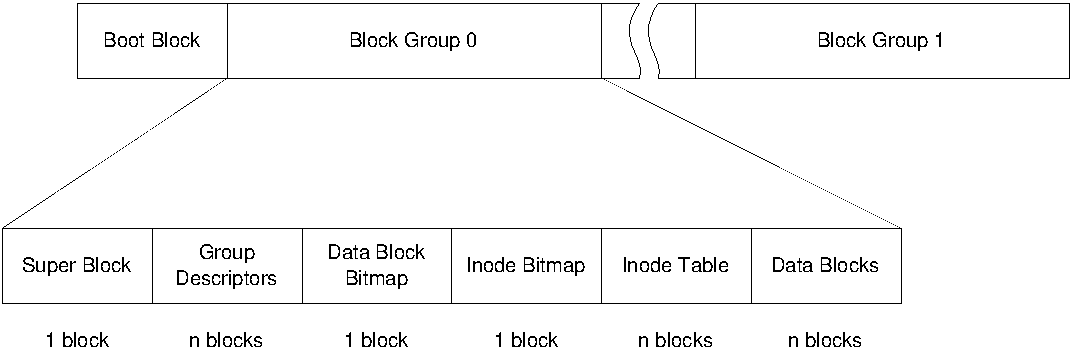
\includegraphics[width=\linewidth]{./files/inc/pic/techRep_ext2_partitionLayout}
\caption{\label{fig:techRep_ext2_partitionLayout}Structure of an Ext2 partition}
\end{center}
\end{figure}

%-----------
\subsection{Super Block}
The Super Block contains all the information about the configuration of the filing system.  The primary copy of the Super Block is stored at an offset of 1024 bytes from the start of the device, and it is essential for mounting the files system.

The information in the Super Block contains fields such as the total number of inodes and blocks in the file system and how many are free, how many inodes and blocks are in each block group, when the file system was mounted (and if it was cleanly unmounted), when it was modified, what version of the file system it is (see the Revisions section below) and which OS created it.

%-----------
\subsection{Inodes}
The inode (index node) is a fundamental concept in the ext2 file system. Each object in the files system is represented by an inode.  The inode structure contains pointers to the file system blocks which contain the data held in the object and all of the metadata about an object except its name. Every inode field is 128 bytes of size. How a file's data blocks is addressed can be seen in figure \ref{fig:techRep_ext2_adressBlocks}.

The metadata about an object includes the permissions, owner, group, flags, size, number of blocks used, access time, change time, modification time, deletion time, number of links, fragments, version (for NFS) and extended attributes (EAs) and/or Access Control Lists (ACLs).


\begin{figure}[H]
\begin{center}
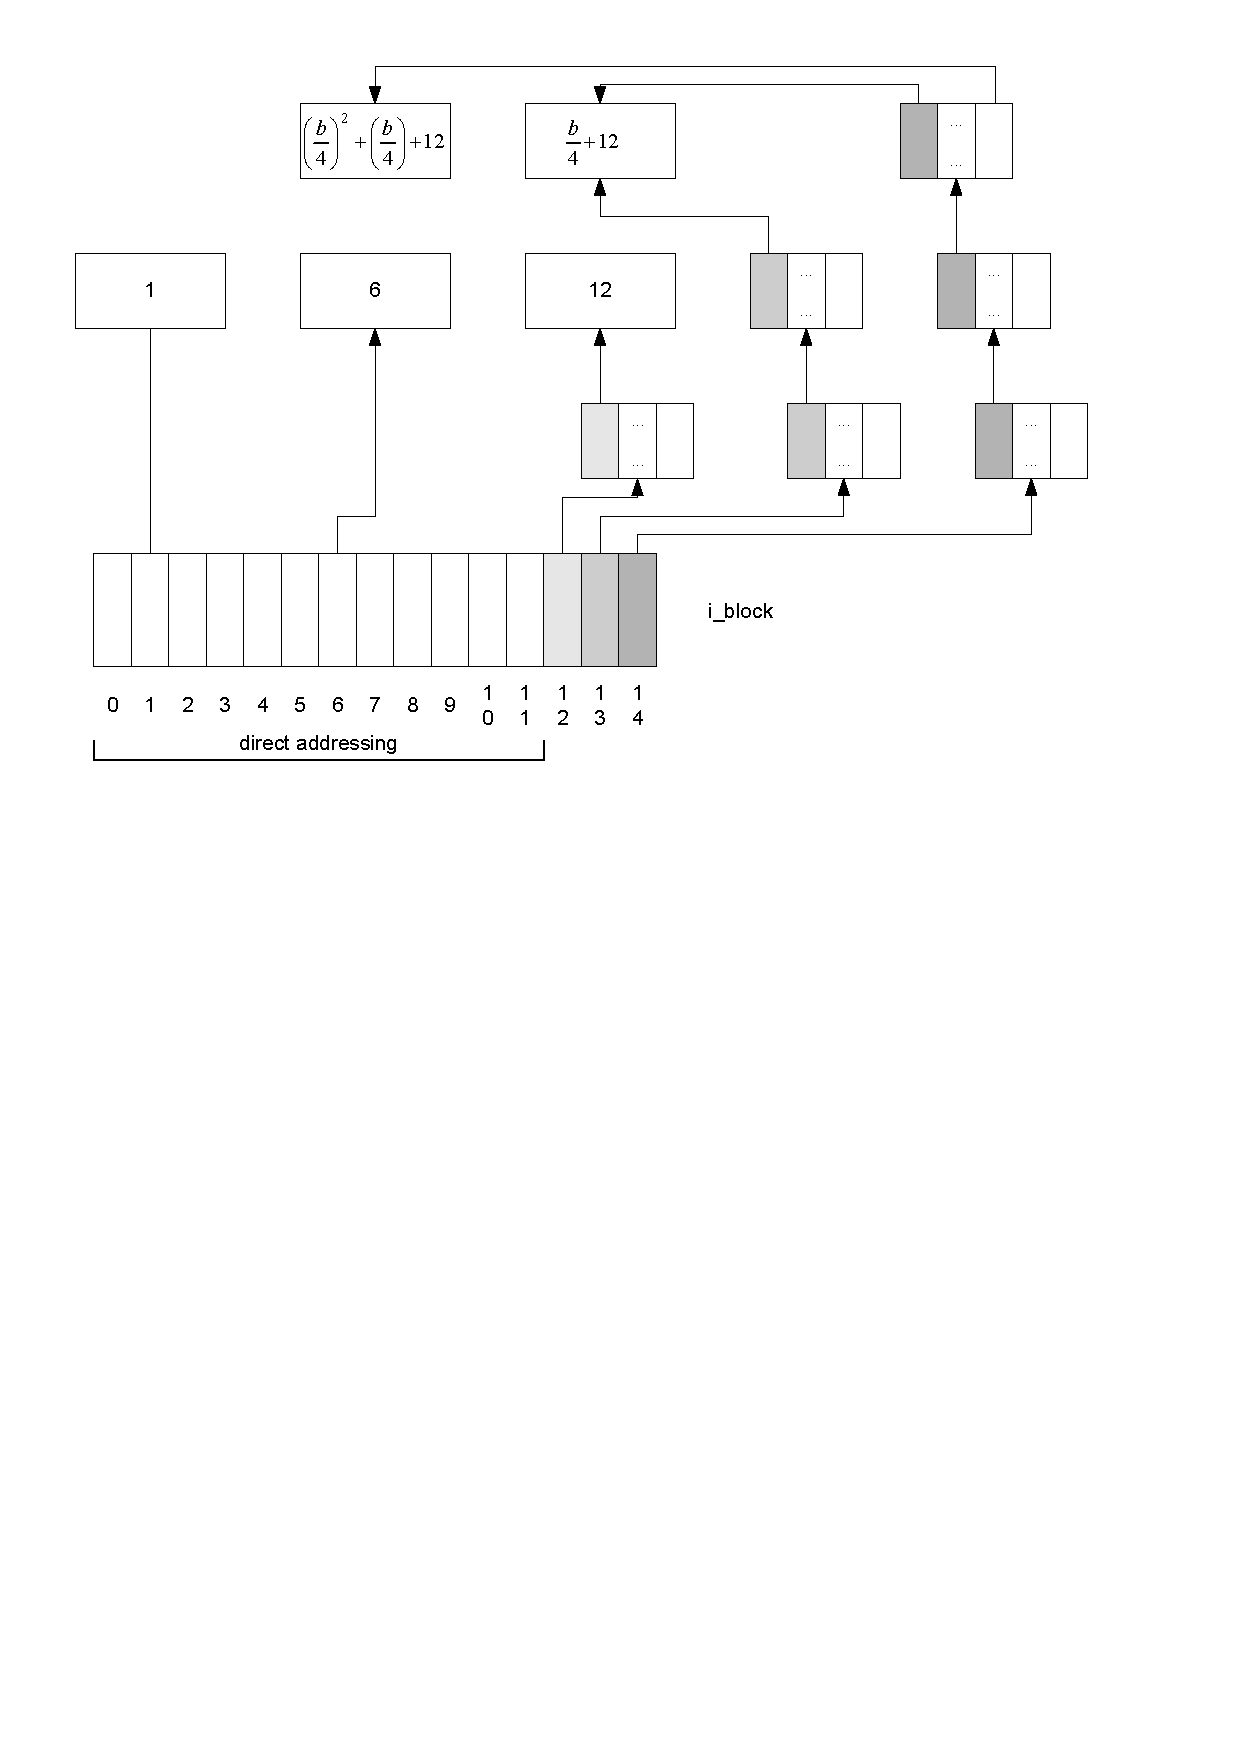
\includegraphics[width=\linewidth]{./files/inc/pic/techRep_ext2_adressBlocks}
\caption{\label{fig:techRep_ext2_adressBlocks}Data structure used to address the file's data block}
\end{center}
\end{figure}

\noindent
There are pointers to the first 12 blocks which contain the file's data in the inode. This mechanism favourites small files. If a file is smaller or equal 12 blocks, it can be addresses directly. If a file is bigger, indirect addressing is used, this means, a file can be retrieved in two disk accesses: One to read the content of the \verb~i-block~ array and one to read the content of the data block itself. For even larger files, three or four consecutive disk accesses are needed to access a data block. (E.g. Component at index 12 contains the logical block number of a block that represents a second-order array of logical block numbers. They correspond to the file block number ranging from $12$ to $\frac{b}{4}+11$ where $b$ is the file system's block size.)

